\newpage
\section{Communication Bluetooth}
\subsection{Matériel à disposition}
Pour ce projet, nous avons pu avoir deux boîtes complètes à disposition. Voici quelques caractéristiques de ce matériel:
\begin{itemize}
	\item SensorTag 1:
	\begin{itemize}
		\item Numéro du capteur: 9
		\item Mac adresse: b0:b4:48:c9:b3:85
		\item Données collectées: Luminosité 
	\end{itemize}
	\item SensorTag 2:
	\begin{itemize}
		\item Numéro du capteur: 16
		\item Mac adresse: b0:b4:48:c9:ba:01
		\item Données collectées: Température, Humidité 
	\end{itemize}
	\item Carte Bluetooth du Waspmote:
	\begin{itemize}
		\item Numéro du socket: 1
	\end{itemize}
\end{itemize}
\subsection{Séquence d'acquisition des données}
Nous avons décidé de collecter les données selon les étapes suivantes dans la boucle principale:
\begin{enumerate}
\item Au lancement de l'application, le module Bluetooth est connecté au socket 1 une seule fois dans la méthode setup.
\item L'application commence par tenter la connexion avec le capteur 1. Si la connexion échoue, l'application passe à la connexion avec le capteur 2 (étape 5).
\item Sinon, une fois le capteur connecté, la période d'acquisition du capteur de luminosité est configurée à 100ms et la mesure est activé. 
\item On attend ensuite 1 seconde, le temps que le capteur fasse quelques mesures. 
\item On va ensuite lire la valeur de la caractéristique et convertir les données. La mesure sur le capteur est ensuite désactivée et l'on se déconnecte du capteur.
\item Les étapes 2 à 5 sont ensuite répétées mais avec le capteur 2 pour récupérer l'humidité et la température.
\end{enumerate}
Toutes les données sont stockées dans des variables globales. Si la connexion avec un des capteurs échoue, ce sont les valeurs précédentes du capteur qui sont envoyée au réseau LoRaWan. L'irrigation d'un champ n'a pas besoin de se faire à la minute près, le fait qu'une des données n'est pas mise à jour pour 5 minutes n'est donc pas dramatique. C'est également pour cela que nous n'avons pas choisi d'utiliser la notification pour recevoir les données des capteurs. L'acquisition des valeurs toutes les 5 minutes est suffisante.\\\\
Les capteurs sont désactivés pour ne plus faire de mesure pendant les 5 minutes d'attente, cela permet d'économiser leur batterie.
\subsubsection{Caractéristiques utilisées}
En nous basant sur le site \url{http://www.ti.com/ww/en/wireless_connectivity/sensortag2015/tearDown.html}, nous avons utilisé le service présenté ci-dessous pour collecter les données du capteur d'humidité. L'avantage est que cette caractéristique donne également la température. On peut avoir les deux valeurs en une seule lecture. 
\begin{figure}[H]
	\begin{center}
		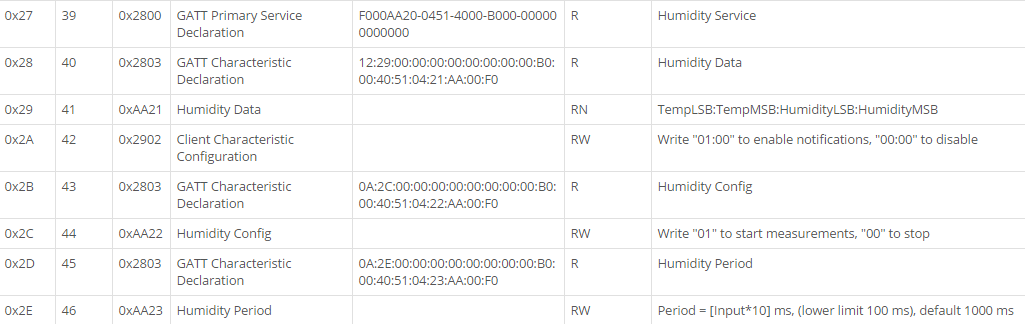
\includegraphics[width=17cm]{img/carhum.png}
		\caption{Caractéristique pour la température et l'humidité}
		\label{humidity}
	\end{center}
\end{figure}
Le service suivant est celui utilisé pour l'acquisition de la luminosité.
\begin{figure}[H]
	\begin{center}
		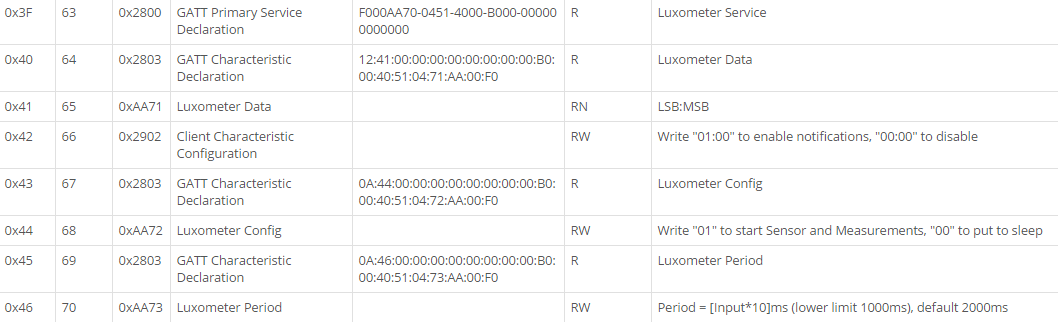
\includegraphics[width=17cm]{img/carlum.png}
		\caption{Caractéristique pour la luminosité}
		\label{luminosity}
	\end{center}
\end{figure}
\textbf{Remarque: }Sur le site cité plus haut, il y a une erreur, le service pour avoir la luminosité qui est présenté n'est pas le bon. Il faut aller dans l'onglet \textit{Full GATT Table} pour voir le vrai luxometer service.\\\\
Le wiki, \url{http://processors.wiki.ti.com/index.php/CC2650_SensorTag_User's_Guide}, a été utilisé pour convertir les données brutes des capteurs dans la bonne unité.\\\\
\textbf{Remarque: }Nous avons remarqué que toutes nos données converties n'avaient aucun sens. Cela est dû à Libellium qui rajoute un byte (le premier, 0) aux données lues par Bluetooth pour indiquer la taille des données à lire. Il faut donc commencer au byte 1 des données reçues pour les convertir. Les valeurs obtenues ont tout de suite plus de sens.
\subsection{Seuils de génération d'alarme}
Le paramètre alarme a une valeur de 0 si tout va bien et de 1 si le champ a besoin d'irrigation. Nous avons fixé trois seuils déclenchant l'alarme:
\begin{itemize}
	\item Si la température est supérieure à 30 degrés
	\item Si le taux d'humidité passe en dessous de 30\%
	\item Si la luminosité est supérieure à 30000 lux. Ce dernier seuil a été fixé selon Wikipédia qui dit que cela correspond à une exposition en plein soleil.
\end{itemize}
\subsection{Attente de 5 minutes}
Nous avons remarqué que les SensorTag n'arrivent pas à rester 5 minutes en advertisement, ils s'éteignent après environ 2 minutes. Cela est très embêtant car nous ne pouvons plus nous connecter avec eux.\\
Afin de résoudre ce problème, nous avons réglé une boucle d'attente qui va se connecter puis se déconnecter à chacun des deux capteurs toutes les minutes pendant 5 minutes. Cela permet de garder les SensorTag éveillés.
\section{Communication LoRaWAN}
Pour la communication LoRaWAN, nous nous sommes basés sur l'exemple \\\textit{LoRaWAN\_08\_join\_otaa\_send\_unconfirmed.pde}. Le join est fait une seule fois au début du programme. Les packets envoyés ne sont pas confirmés. Nous avons configuré notre \textit{Device EUI} comme étant 11-12-13-14-15-16-17-18\\\\
Une fois les données des capteurs collectées, elles sont regroupées dans une seule trame au format JSON. La trame créée est ensuite convertie en sa représentation ASCII hexadécimale, car le récepteur n'accepte pas d'autre format. Puis on termine par l'envoi de la trame et l'on recommence le tout après 5 minutes.
\subsection{Tests de la communication}
Voici une capture d'écran du moniteur série de Waspmote. On voit que l'on rejoint le réseau, collecte des données et qu'un envoi est fait.
\begin{figure}[H]
	\begin{center}
		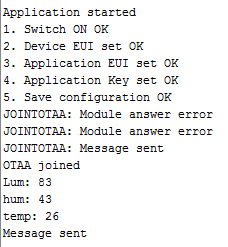
\includegraphics[width=6cm]{img/console.png}
		\caption{Moniteur série de Waspmote}
		\label{Moniteur}
	\end{center}
\end{figure}
Toutes les données envoyées sont visibles dans la fenêtre de debug\\ (http://192.168.32.4/debug\_window.php). Les packets que nous avons envoyés sont encadrés en rouge. On voit que les cinq minutes entre les trames sont bien respectées, on est à 5 minutes et environ 14 secondes entre chaque envoi. 
\begin{figure}[H]
	\begin{center}
		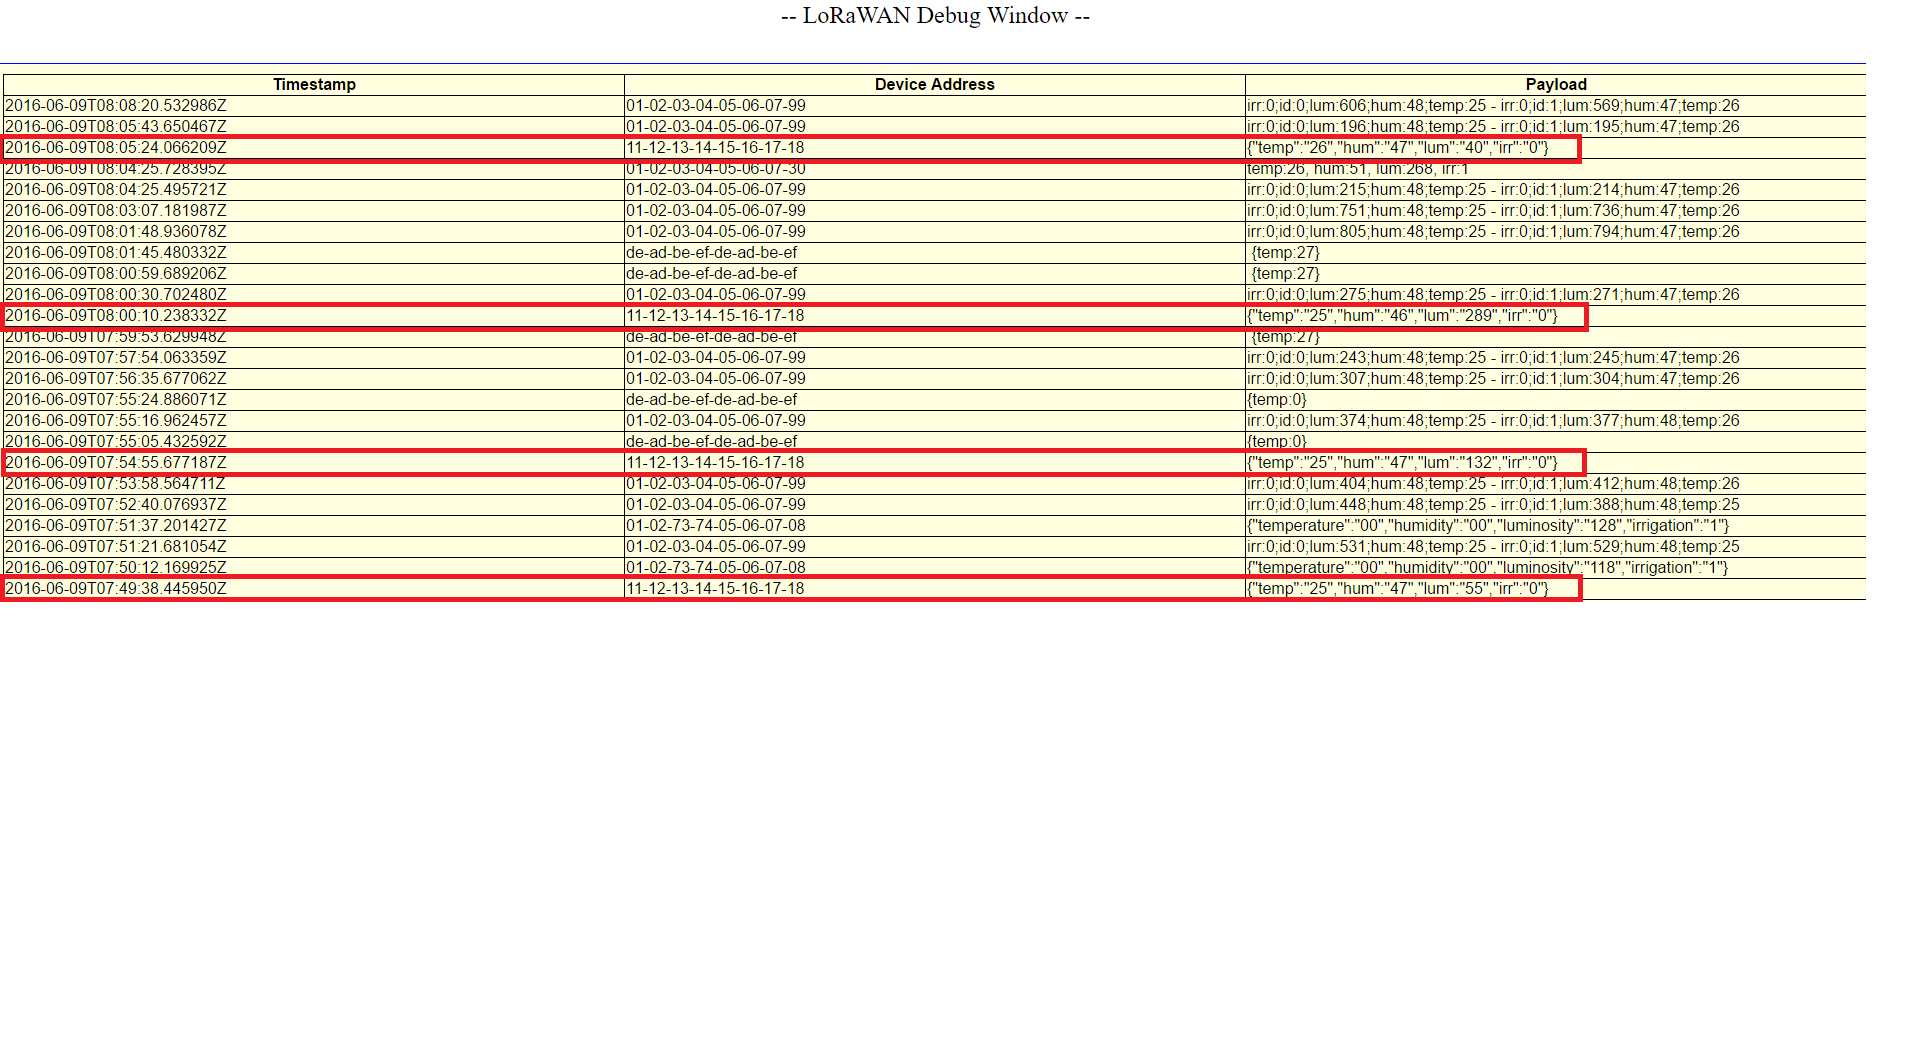
\includegraphics[width=17cm]{img/result.png}
		\caption{Réception des packets}
		\label{debug}
	\end{center}
\end{figure}